% Created 2022-06-29 Wed 01:10
% Intended LaTeX compiler: pdflatex
\documentclass[letterpaper, 12pt]{report}
\usepackage[utf8]{inputenc}
\usepackage[T1]{fontenc}
\usepackage{graphicx}
\usepackage{longtable}
\usepackage{wrapfig}
\usepackage{rotating}
\usepackage[normalem]{ulem}
\usepackage{amsmath}
\usepackage{amssymb}
\usepackage{capt-of}
\usepackage{hyperref}
\usepackage{amsmath}		% Extra math definitions
\usepackage{graphics}		% PostScript figures
\usepackage{setspace}		% 1.5 spacing
\usepackage{longtable}          % Tables spanning pages
\usepackage{natbib}
\usepackage{times}
\usepackage{url}
\usepackage{latexsym}
\usepackage[usenames]{color}
\usepackage{covington}
\usepackage{graphicx}
\usepackage{multirow}
\usepackage{subcaption}%#+LATEX_HEADER: \usepackage{subfigure}
\usepackage{booktabs}
\usepackage{tabularx}
\usepackage[T1]{fontenc}
\usepackage[utf8]{inputenc}
\usepackage[english]{babel}
\usepackage{blindtext}
\usepackage{amsfonts}
\usepackage{amsthm}
\usepackage[table,xcdraw]{xcolor}
\usepackage{rotating}
\usepackage{listings}
\definecolor{NiceBlue}{RGB}{11, 102, 163}
\definecolor{SlightRed}{RGB}{249,38,114}
\usepackage{textcomp} % other glyphs needed for upquote in listings below
\lstdefinelanguage{DemoExample}
{ basicstyle=\footnotesize \ttfamily,
commentstyle=\color{SlightRed} \rmfamily\itshape,
stringstyle=\color{NiceBlue},
morecomment=[s]{/*}{*/},
morestring=[b]'
}
\usepackage[fancyhdr]{macros/McECEThesis}	% Thesis style
\usepackage{McGillLogo}		% McGill University crest
\usepackage{color}
\insidemargin = 1.1in
\outsidemargin = 1.1in
\abovemargin = 1.1in
\belowmargin = 0.75in
\newcommand{\beq}{\begin{equation}}
\newcommand{\eeq}{\end{equation}}
\usepackage{palatino}           % Less abusive fonts
\usepackage{macros/palatcm}
\usepackage{hyperref}
\let\mathexp=\exp %redefine \exp to \mathexp cuz gb4e package redefines \exp
\usepackage{gb4e}
\noautomath
\usepackage[acronym,toc,section=section]{glossaries}
\makeglossaries
\newglossaryentry{tlm}{name=Transformers,description={{A class of models first derived by Vaswani et al. 2017}}}
\newacronym{llm}{LLMs}{Large Language Models}
\newacronym{qos}{QoS}{quality-of-service}
\newacronym{bb}{BB}{branch and bound}
\author{Koustuv Sinha}
\date{}
\title{PhD Thesis}
\hypersetup{
 pdfauthor={Koustuv Sinha},
 pdftitle={PhD Thesis},
 pdfkeywords={},
 pdfsubject={},
 pdfcreator={Emacs 28.1 (Org mode 9.6)}, 
 pdflang={English}}
\begin{document}

\maketitle
\raggedbottom
\spacing{1.5}%\onehalfspacing
\pagenumbering{roman}

\chapter*{Acknowledgements}
\label{sec:orgecdfd06}
\chapter*{Abstract}
\label{sec:org5f97da3}
\chapter*{Abstract in French}
\label{sec:org0716849}
\chapter*{Contributions to Original Knowledge}
\label{sec:orge1b928a}
\chapter*{Contributions of Authors}
\label{sec:org67e36a0}
\listoffigures{}

\chapter*{List of Tables}
\label{sec:orge4be181}
\clearpage
\setcounter{tocdepth}{3}
\tableofcontents

\clearpage

\pagenumbering{arabic}
\chapter{Introduction}
\label{sec:org84b1781}
\textbf{\textbf{Central Theme of the thesis}} : Understanding systematicity in pre-trained language models through semantic and syntactic generalization.

In this thesis I discuss my work on understanding systematicity in pre-trained language models.

\clearpage
\chapter{Background}
\label{sec:orge973dec}



\section{Early methods for text representation}
\label{sec:org36095ba}
\section{Neural Inductive bias of text representation}
\label{sec:org1962e2d}
\subsection{Feed Forward Neural Networks}
\label{sec:org0a7045d}
\subsection{Recurrent Neural Networks}
\label{sec:org768a21d}
\subsection{Transformer Models}
\label{sec:org16f1a22}

\gls{llm} are the state-of-the-art in language models, which are based on \gls{tlm}.
\section{Pre-training and the advent of Large Language Models}
\label{sec:org7274d30}
Success of pre-training and scale
\section{Systematicity and Generalization}
\label{sec:orgcf6e128}
\subsection{Definitions}
\label{sec:orga318eb1}
\begin{enumerate}
\item Productivity
\label{sec:orge58aa17}
\item Word Order Sensitivity
\label{sec:org8020cf9}
\end{enumerate}
\subsection{Tasks}
\label{sec:org6657ae7}
\clearpage
\chapter{Understanding semantic generalization through productivity}
\label{sec:orgcc5df70}

\section{Technical Background}
\label{sec:org6187e60}
\section{CLUTRR: A Diagnostic Benchmark for Inductive Reasoning in Text}
\label{sec:orgd01b38f}

Paper: \cite{sinha2019a}

\subsection{Dataset construction}
\label{sec:org704afa9}

\begin{figure}[htbp]
\centering
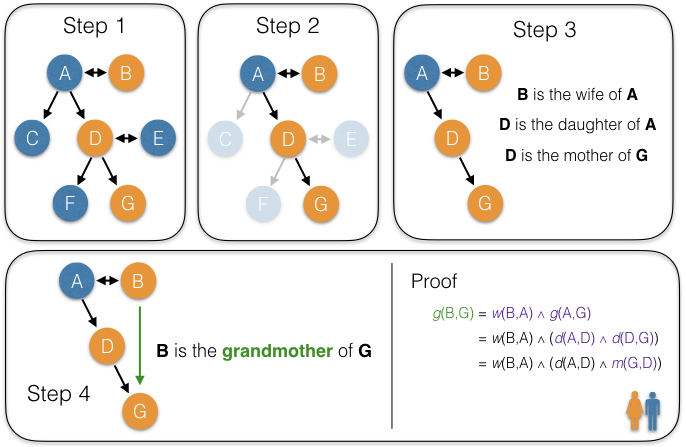
\includegraphics[height=0.3\textwidth]{figs/clutrr/dataset_const_proof.png}
\caption{Dataset generation pipeline.}
\end{figure}

\begin{figure}[htbp]
\centering
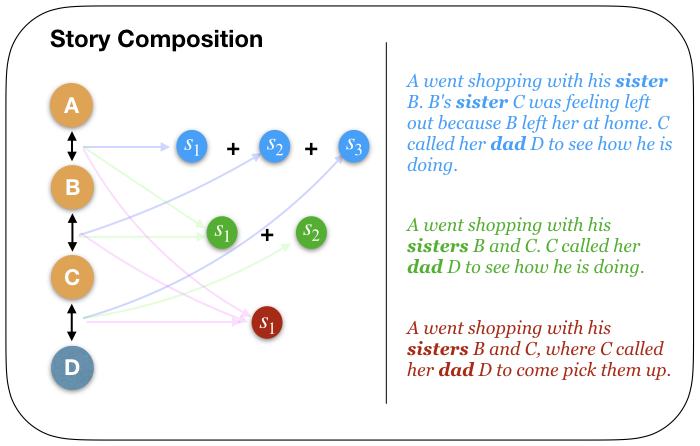
\includegraphics[height=0.3\textwidth]{figs/clutrr/composition.png}
\caption{Illustration of how a set of facts can split and combined in various ways across sentences.}
\end{figure}

\begin{figure}[htbp]
\centering
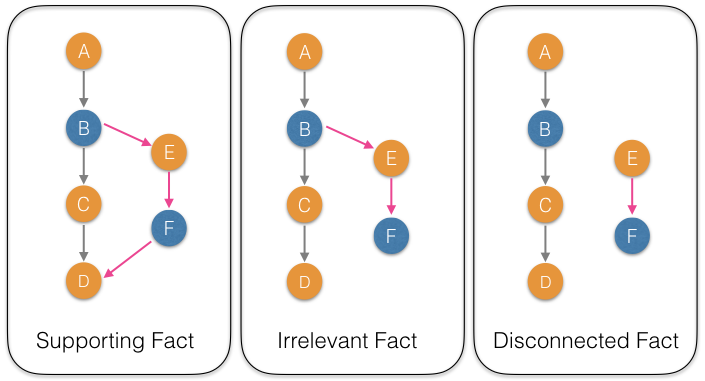
\includegraphics[height=0.3\textwidth]{figs/clutrr/clutrr_noise.png}
\caption{Noise generation procedures of CLUTRR.}
\end{figure}

\subsection{Productivity and reasoning}
\label{sec:orgefd9eef}
\section{Results}
\label{sec:org8bb5b76}

\begin{center}
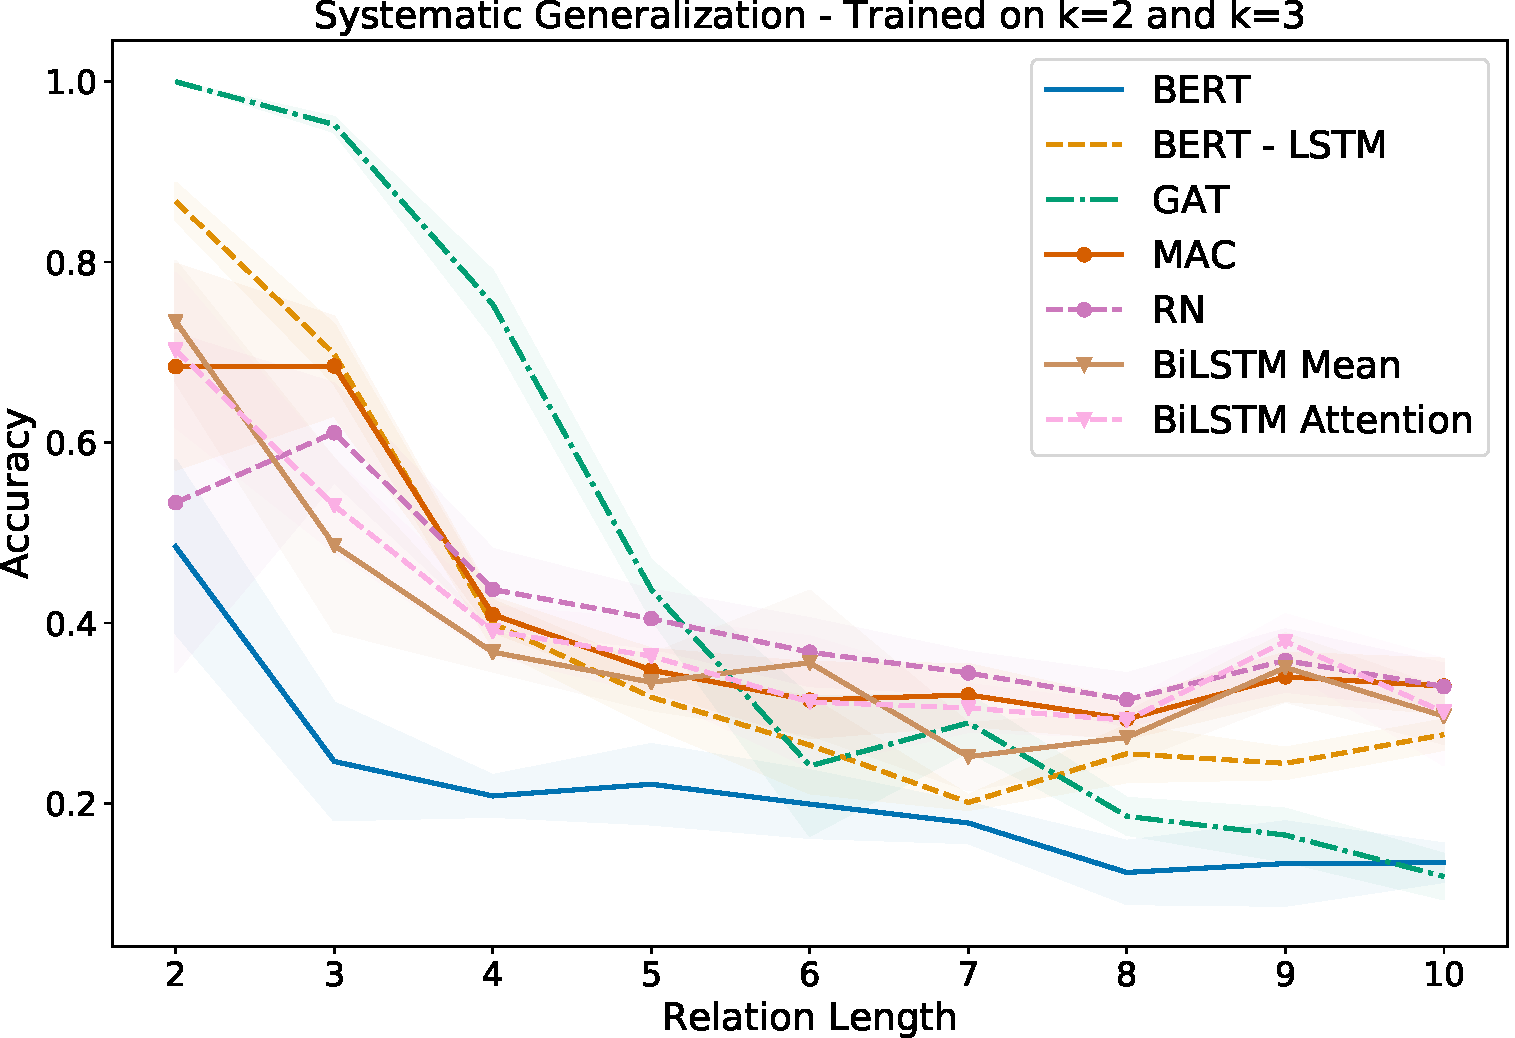
\includegraphics[height=0.3\textwidth]{figs/clutrr/emnlp/sys_gen_23.pdf}
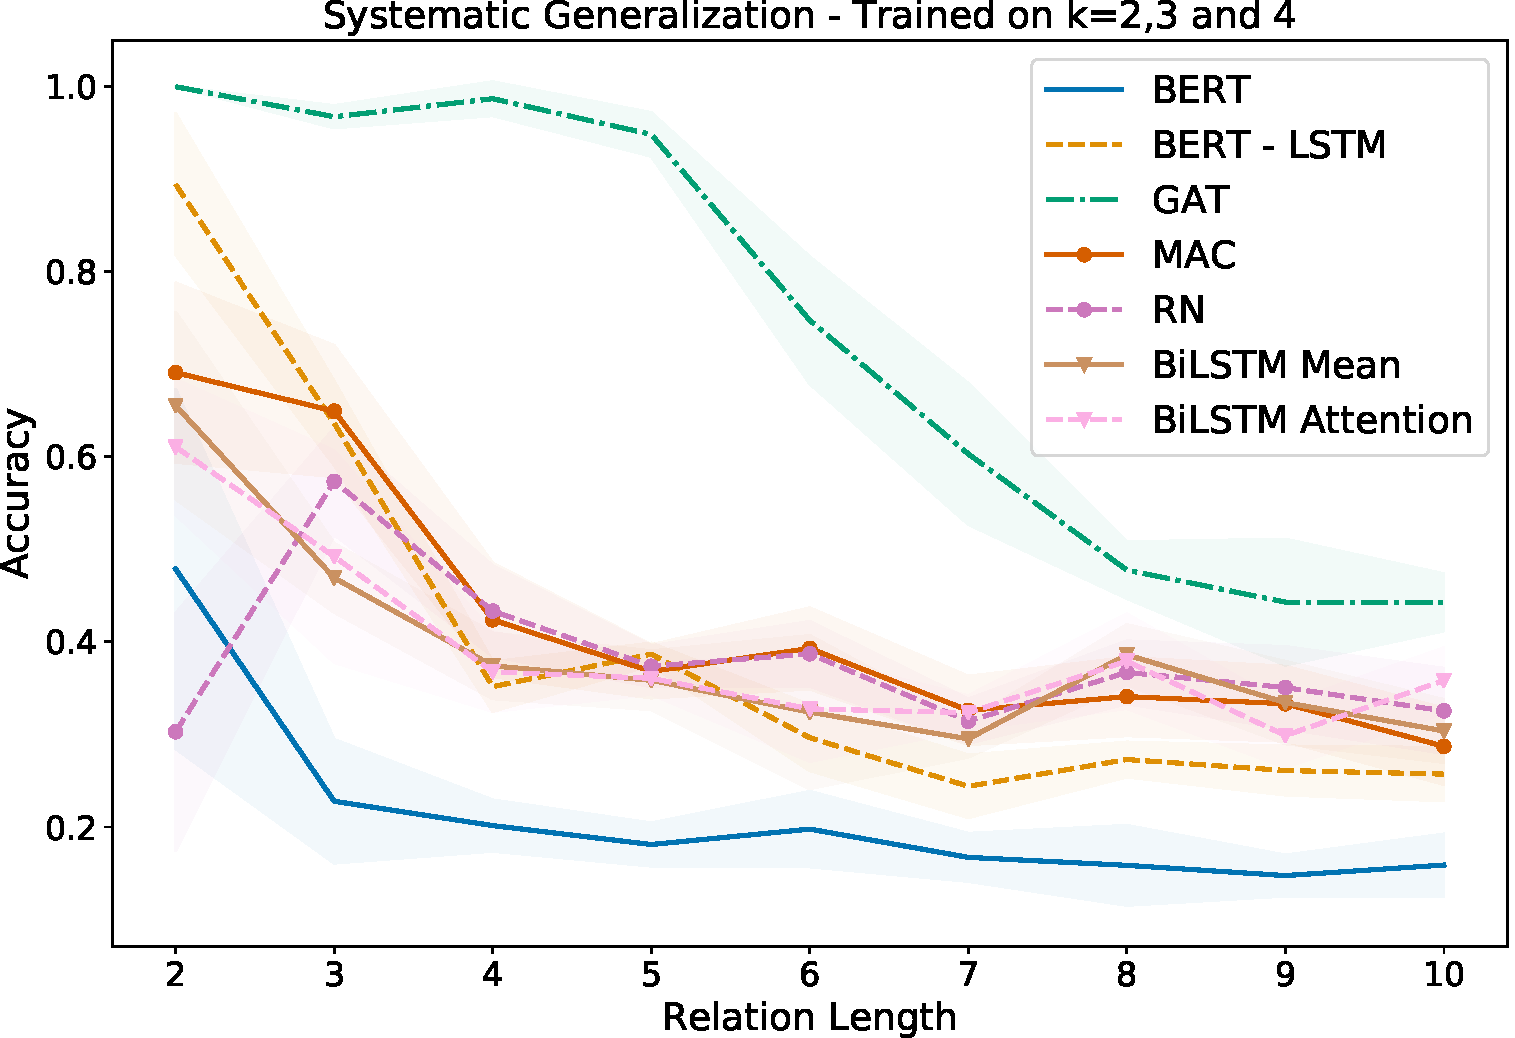
\includegraphics[height=0.3\textwidth]{figs/clutrr/emnlp/sys_gen_234.pdf}
\end{center}
\begin{figure}[htbp]
\centering

\includegraphics[height=0.0001in]{figs/empy_fig.png}
\caption{Systematic generalization when train on k=\(2\) and \(3\).}
\end{figure}


\section{Related Work}
\label{sec:org777df69}
\section{Discussion}
\label{sec:orgb3a0d20}
\section{Follow-up findings in the community}
\label{sec:org89d09b3}
\clearpage
\chapter{Quantifying syntactic generalization using word order}
\label{sec:org4093e01}

Paper \cite{sinha2021a}

\section{Technical Background}
\label{sec:org27e141c}
\section{Word Order in Natural Language Inference}
\label{sec:org0bc8be0}
\subsection{Probe Construction}
\label{sec:org0679257}

\begin{figure}[htbp]
\centering
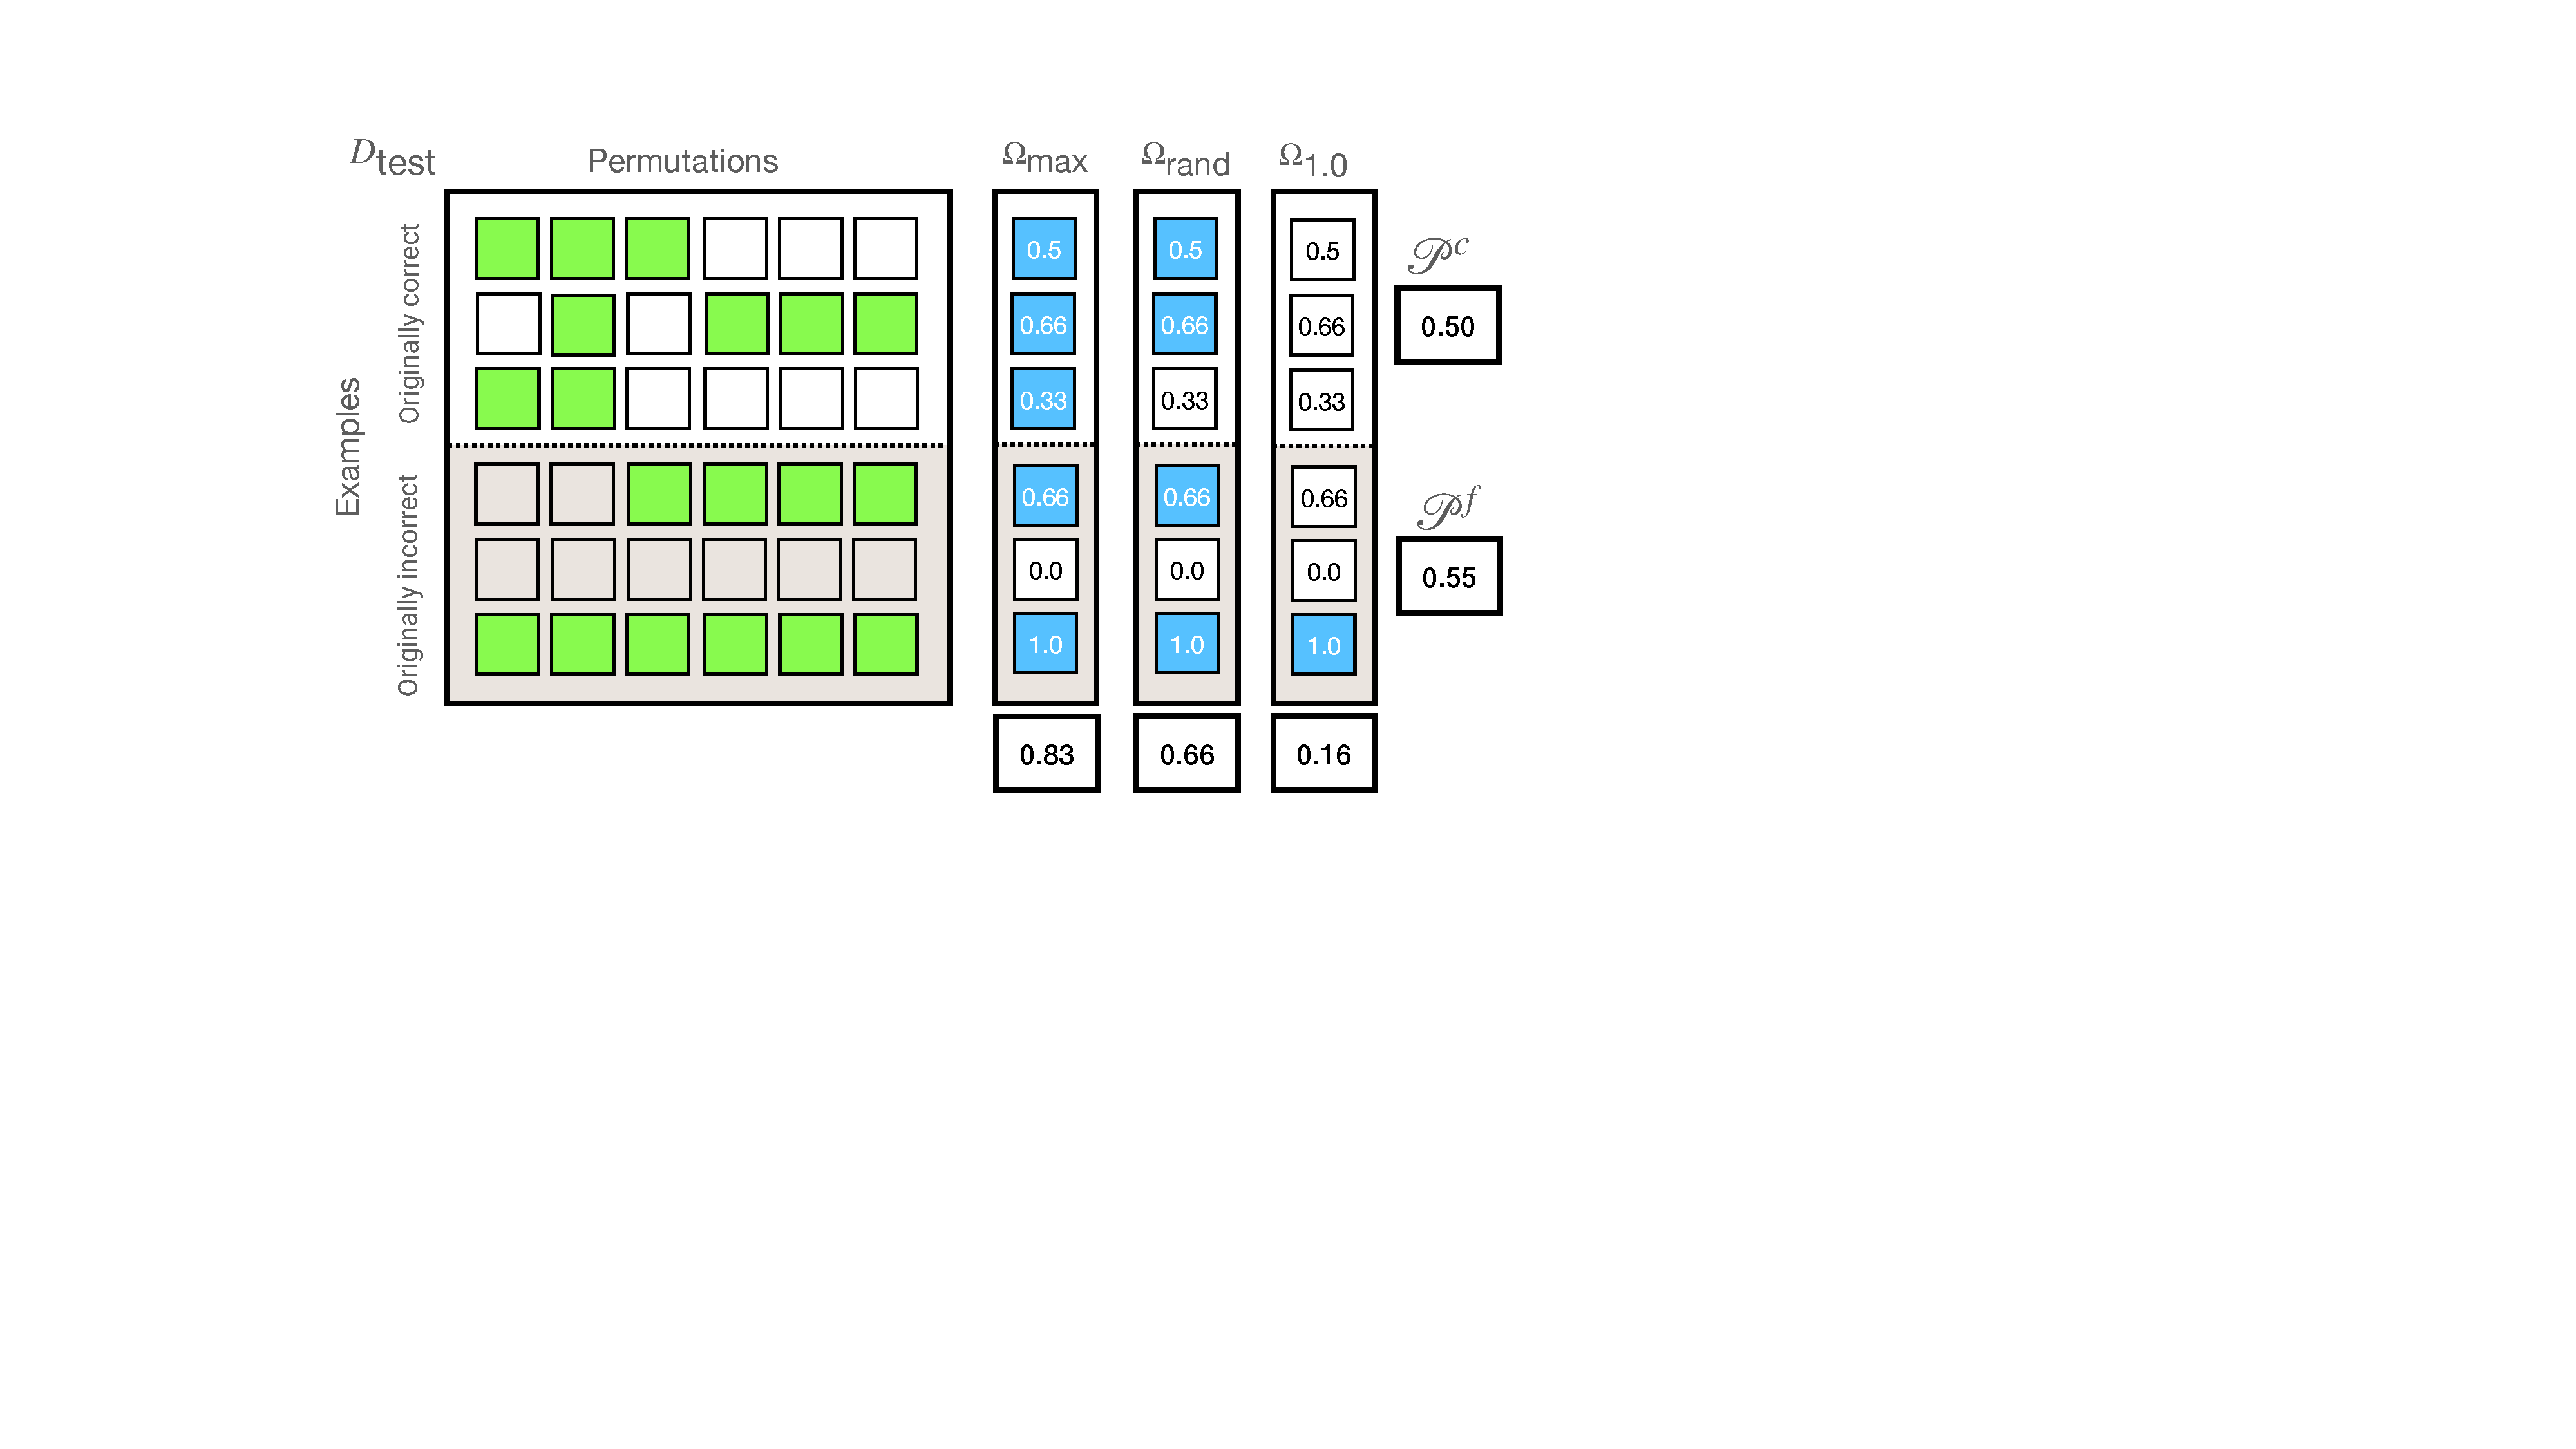
\includegraphics[height=0.3\textwidth]{figs/unli/nli_gen_perm_desc.pdf}
\caption{Graphical representation of the Permutation Acceptance class of metrics.}
\end{figure}

\section{Experiments \& Results}
\label{sec:org86be1bc}

\begin{figure}[htbp]
\centering
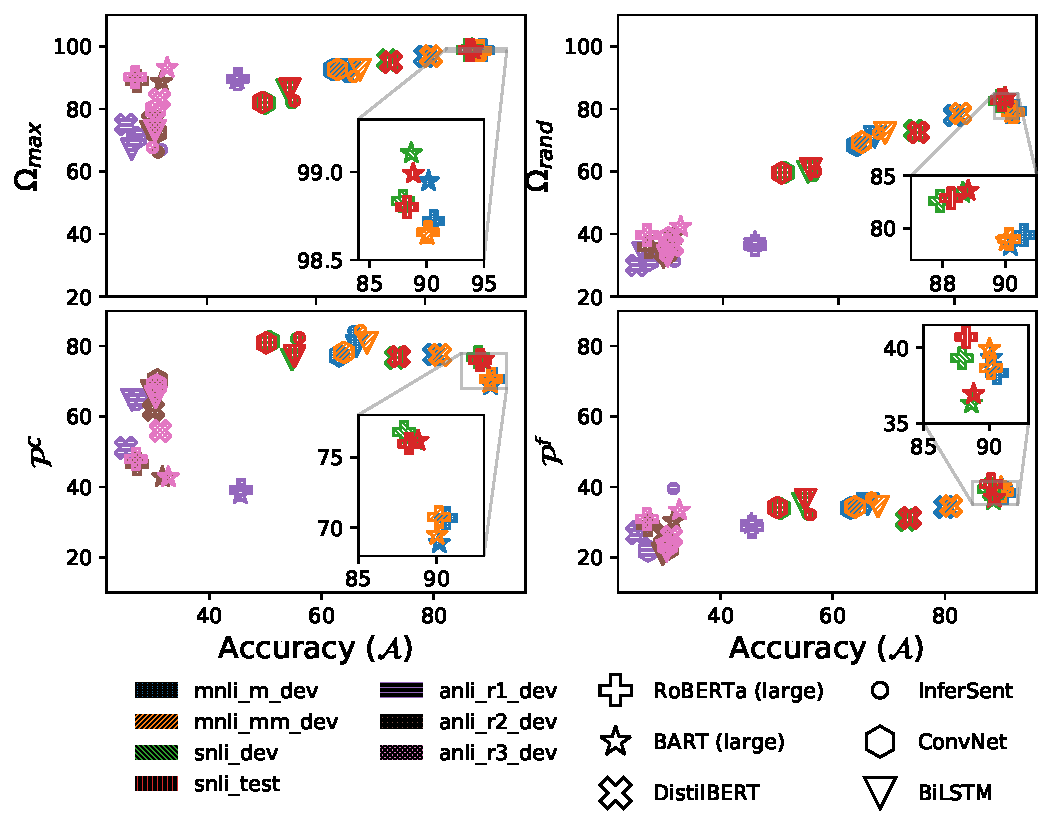
\includegraphics[width=.9\linewidth]{figs/unli/comb_plot_all.pdf}
\caption{Comparison of \(\omega_{\text{max}}\), \(\omega_{\text{rand}}\), \(\mathcal{P}^{c}\) and \(\mathcal{P}^{f}\) with the model accuracy \(\mathcal{A}\) on multiple datasets, where all models are trained on the MNLI corpus \cite{williams-etal-2018-broad}.}
\end{figure}

\begin{figure}[htbp]
\centering
\includegraphics[width=.9\linewidth]{figs/unli/all_entropy.png}
\caption{Average entropy of model confidences on permutations..}
\end{figure}

\begin{figure}[htbp]
\centering
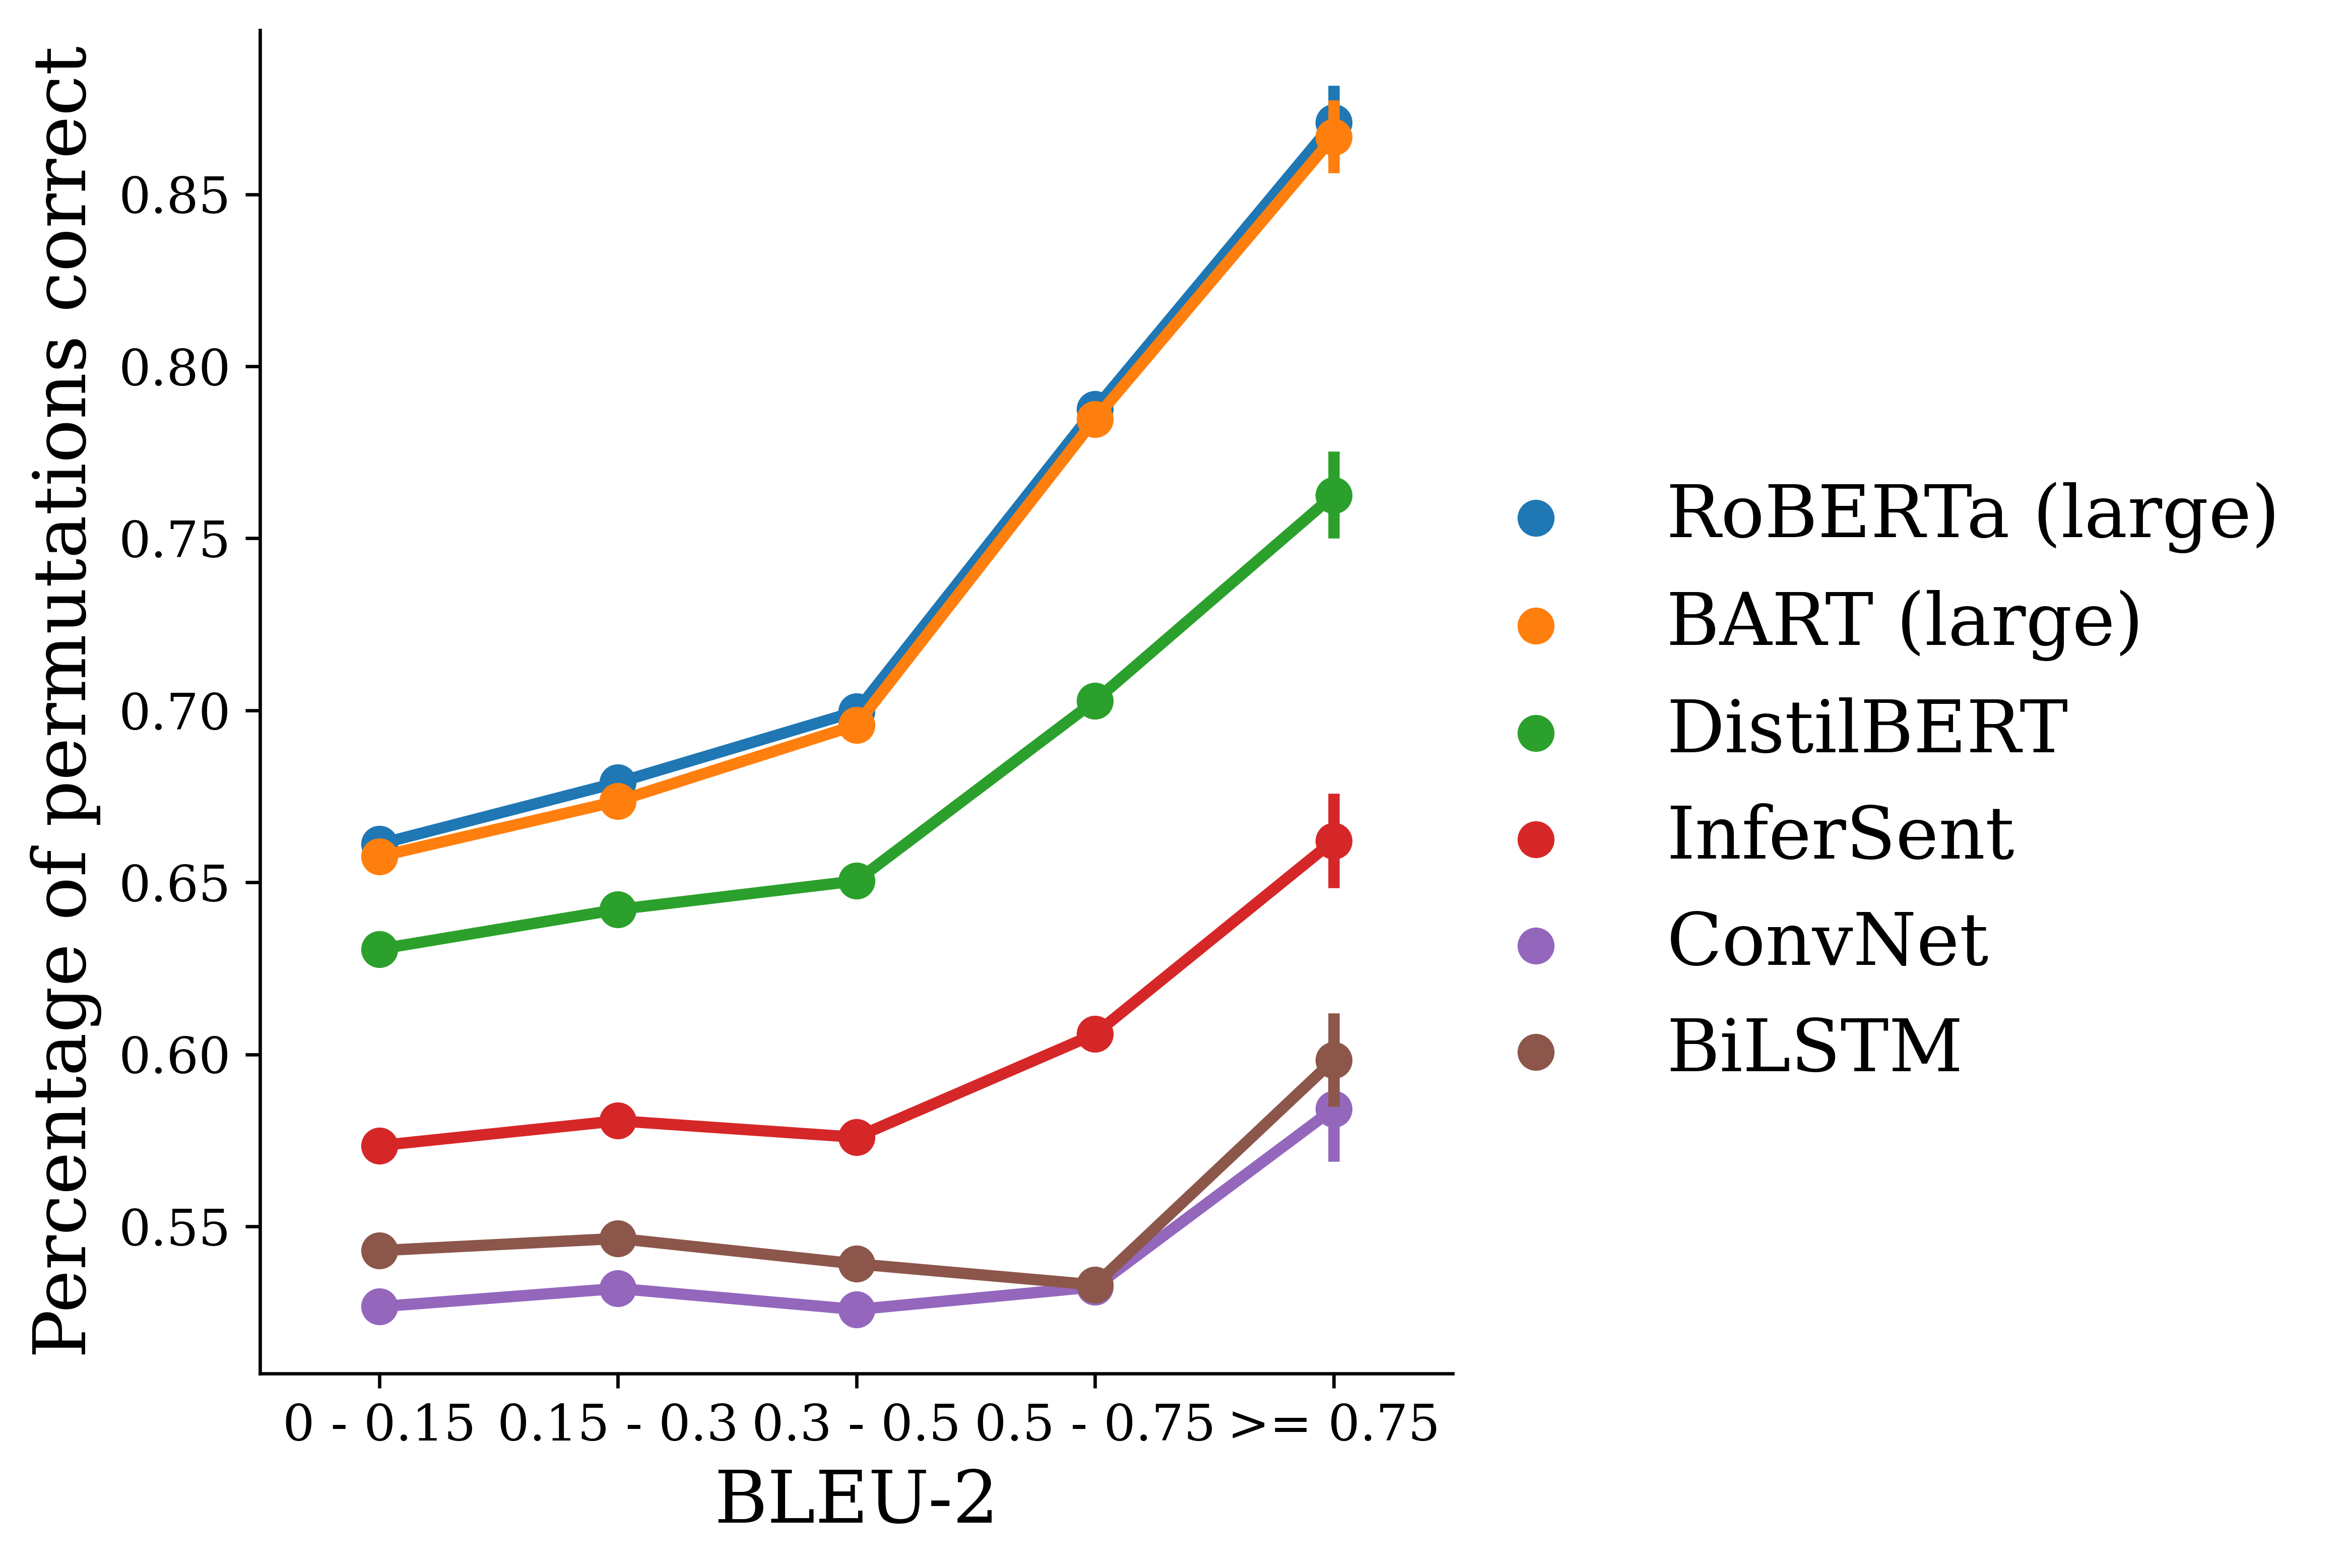
\includegraphics[width=.9\linewidth]{figs/unli/bleu_2_all.png}
\caption{BLEU-2 score versus acceptability of permuted sentences across all test datasets.}
\end{figure}

\begin{figure}[htbp]
\centering
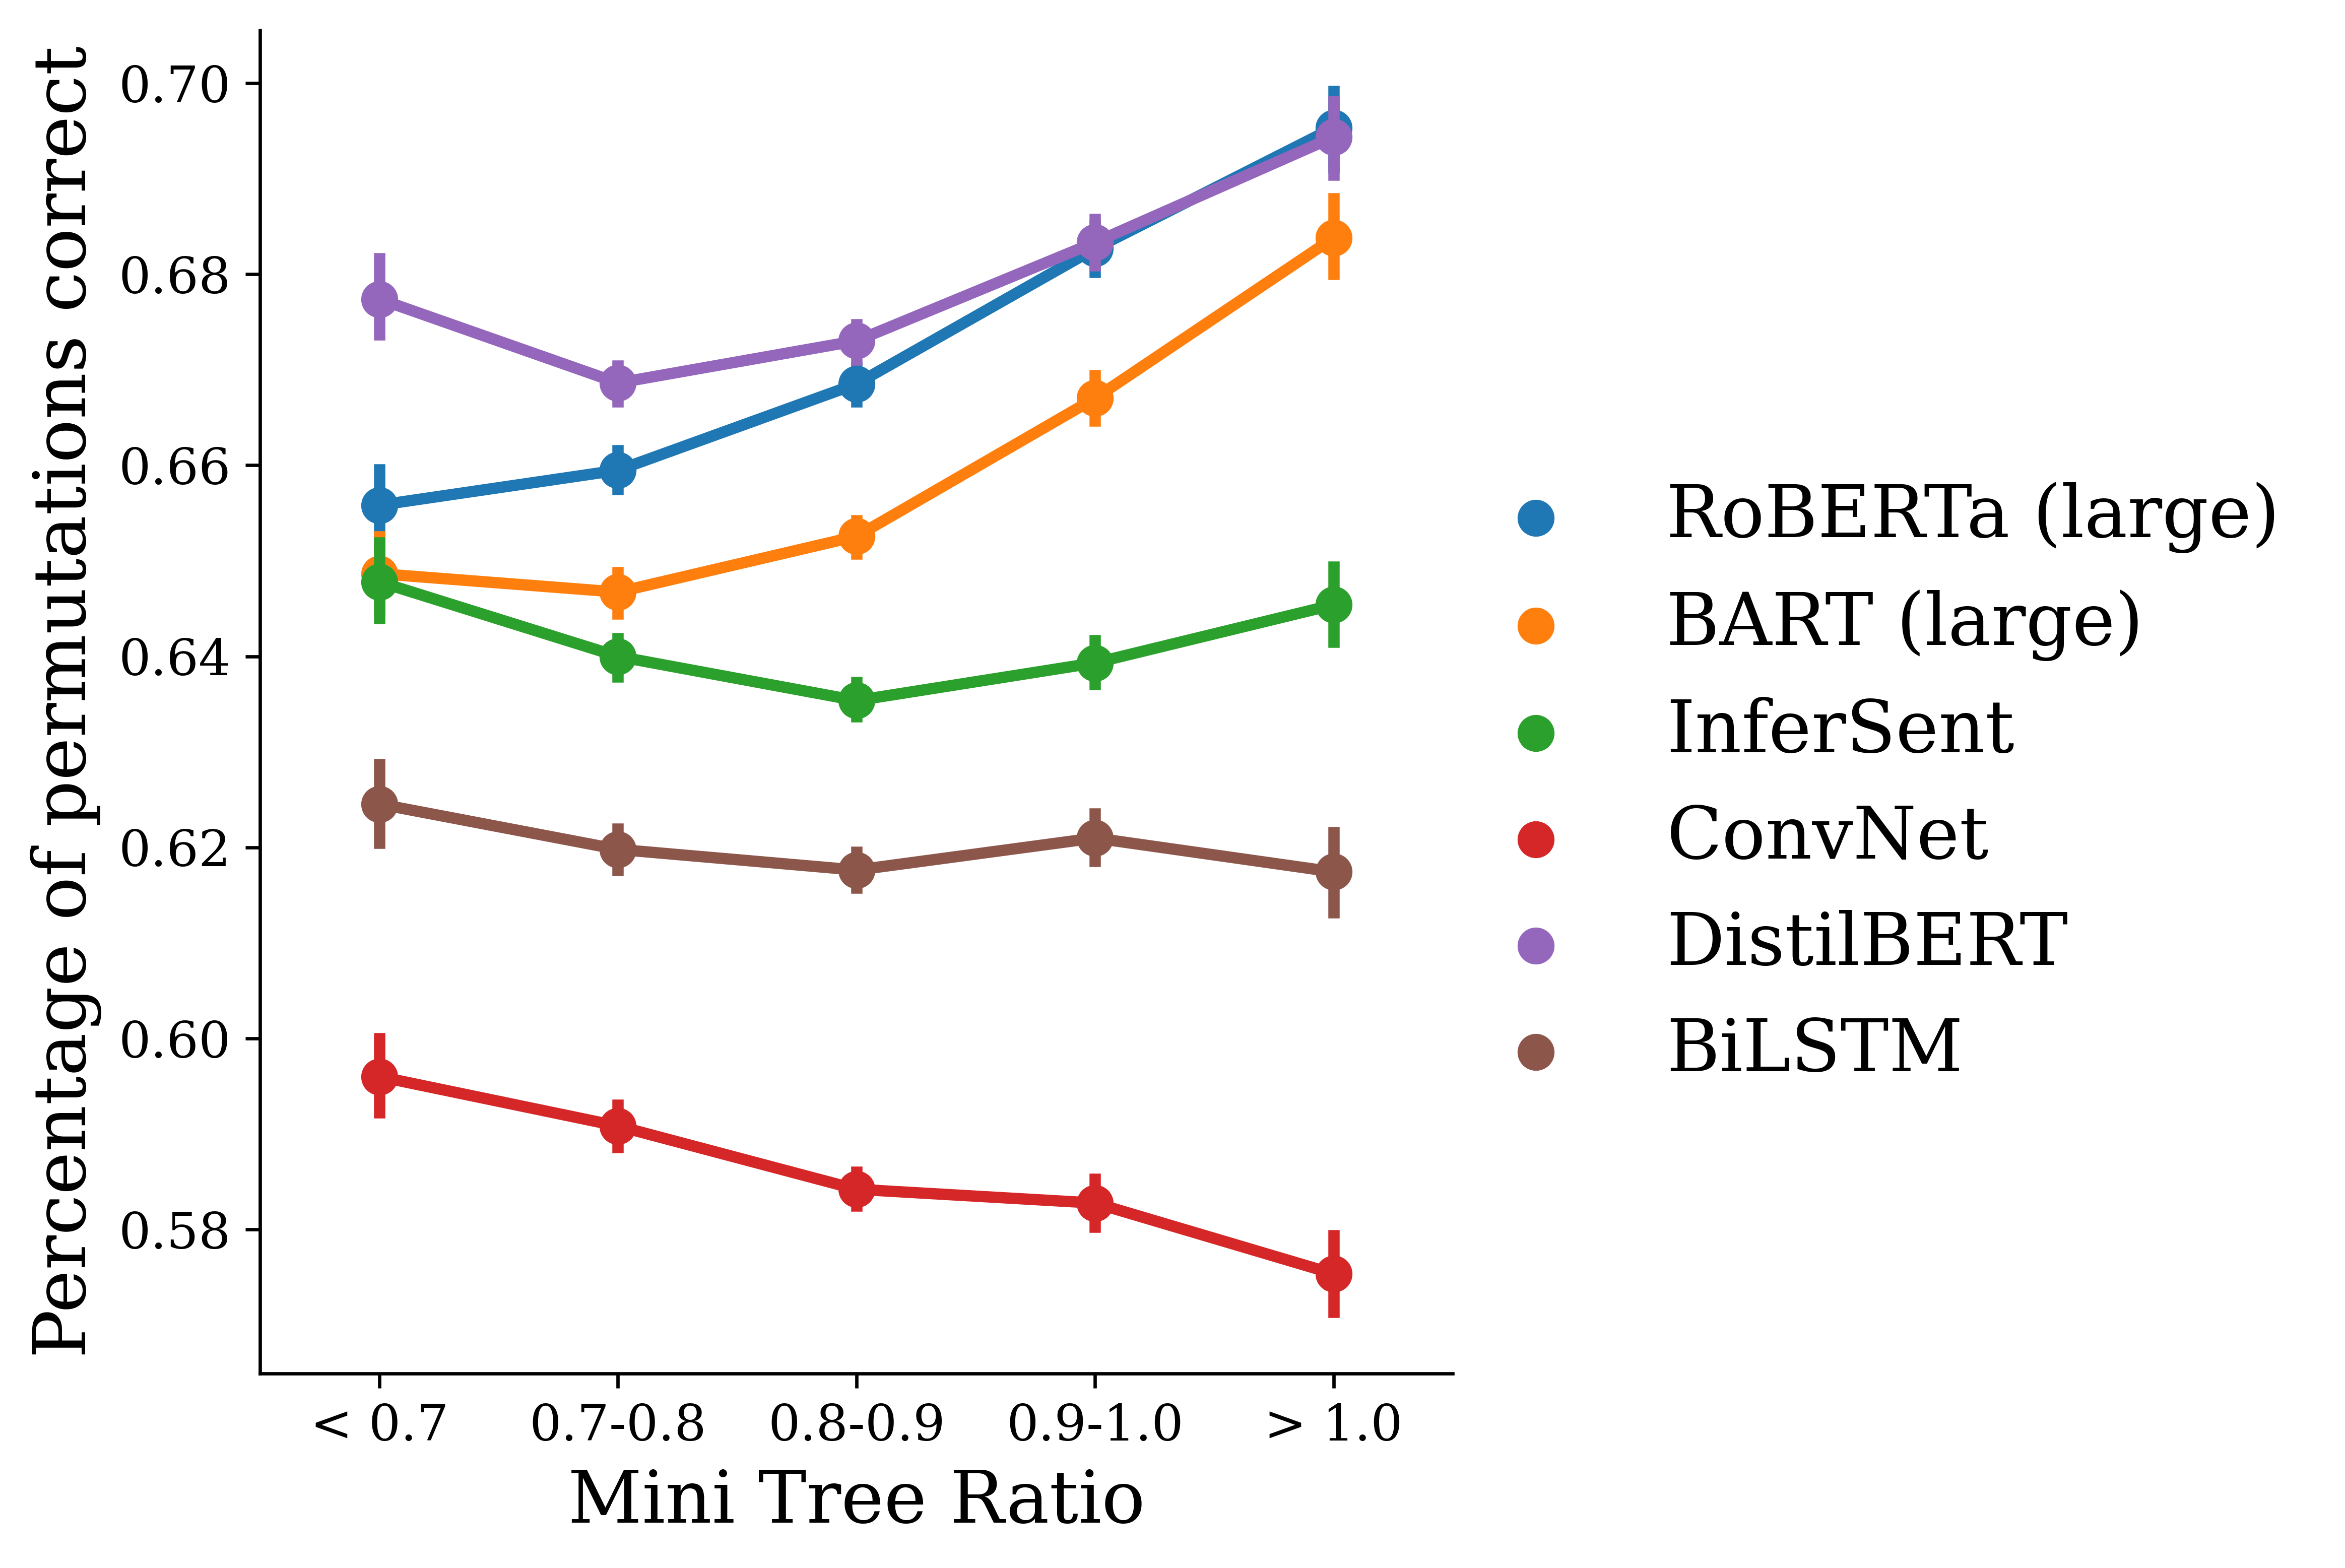
\includegraphics[width=.9\linewidth]{figs/unli/min_tree_4.png}
\caption{POS Tag Mini-Tree overlap score and percentage of permutations which the models assigned the gold label.}
\end{figure}

\begin{figure}[htbp]
\centering
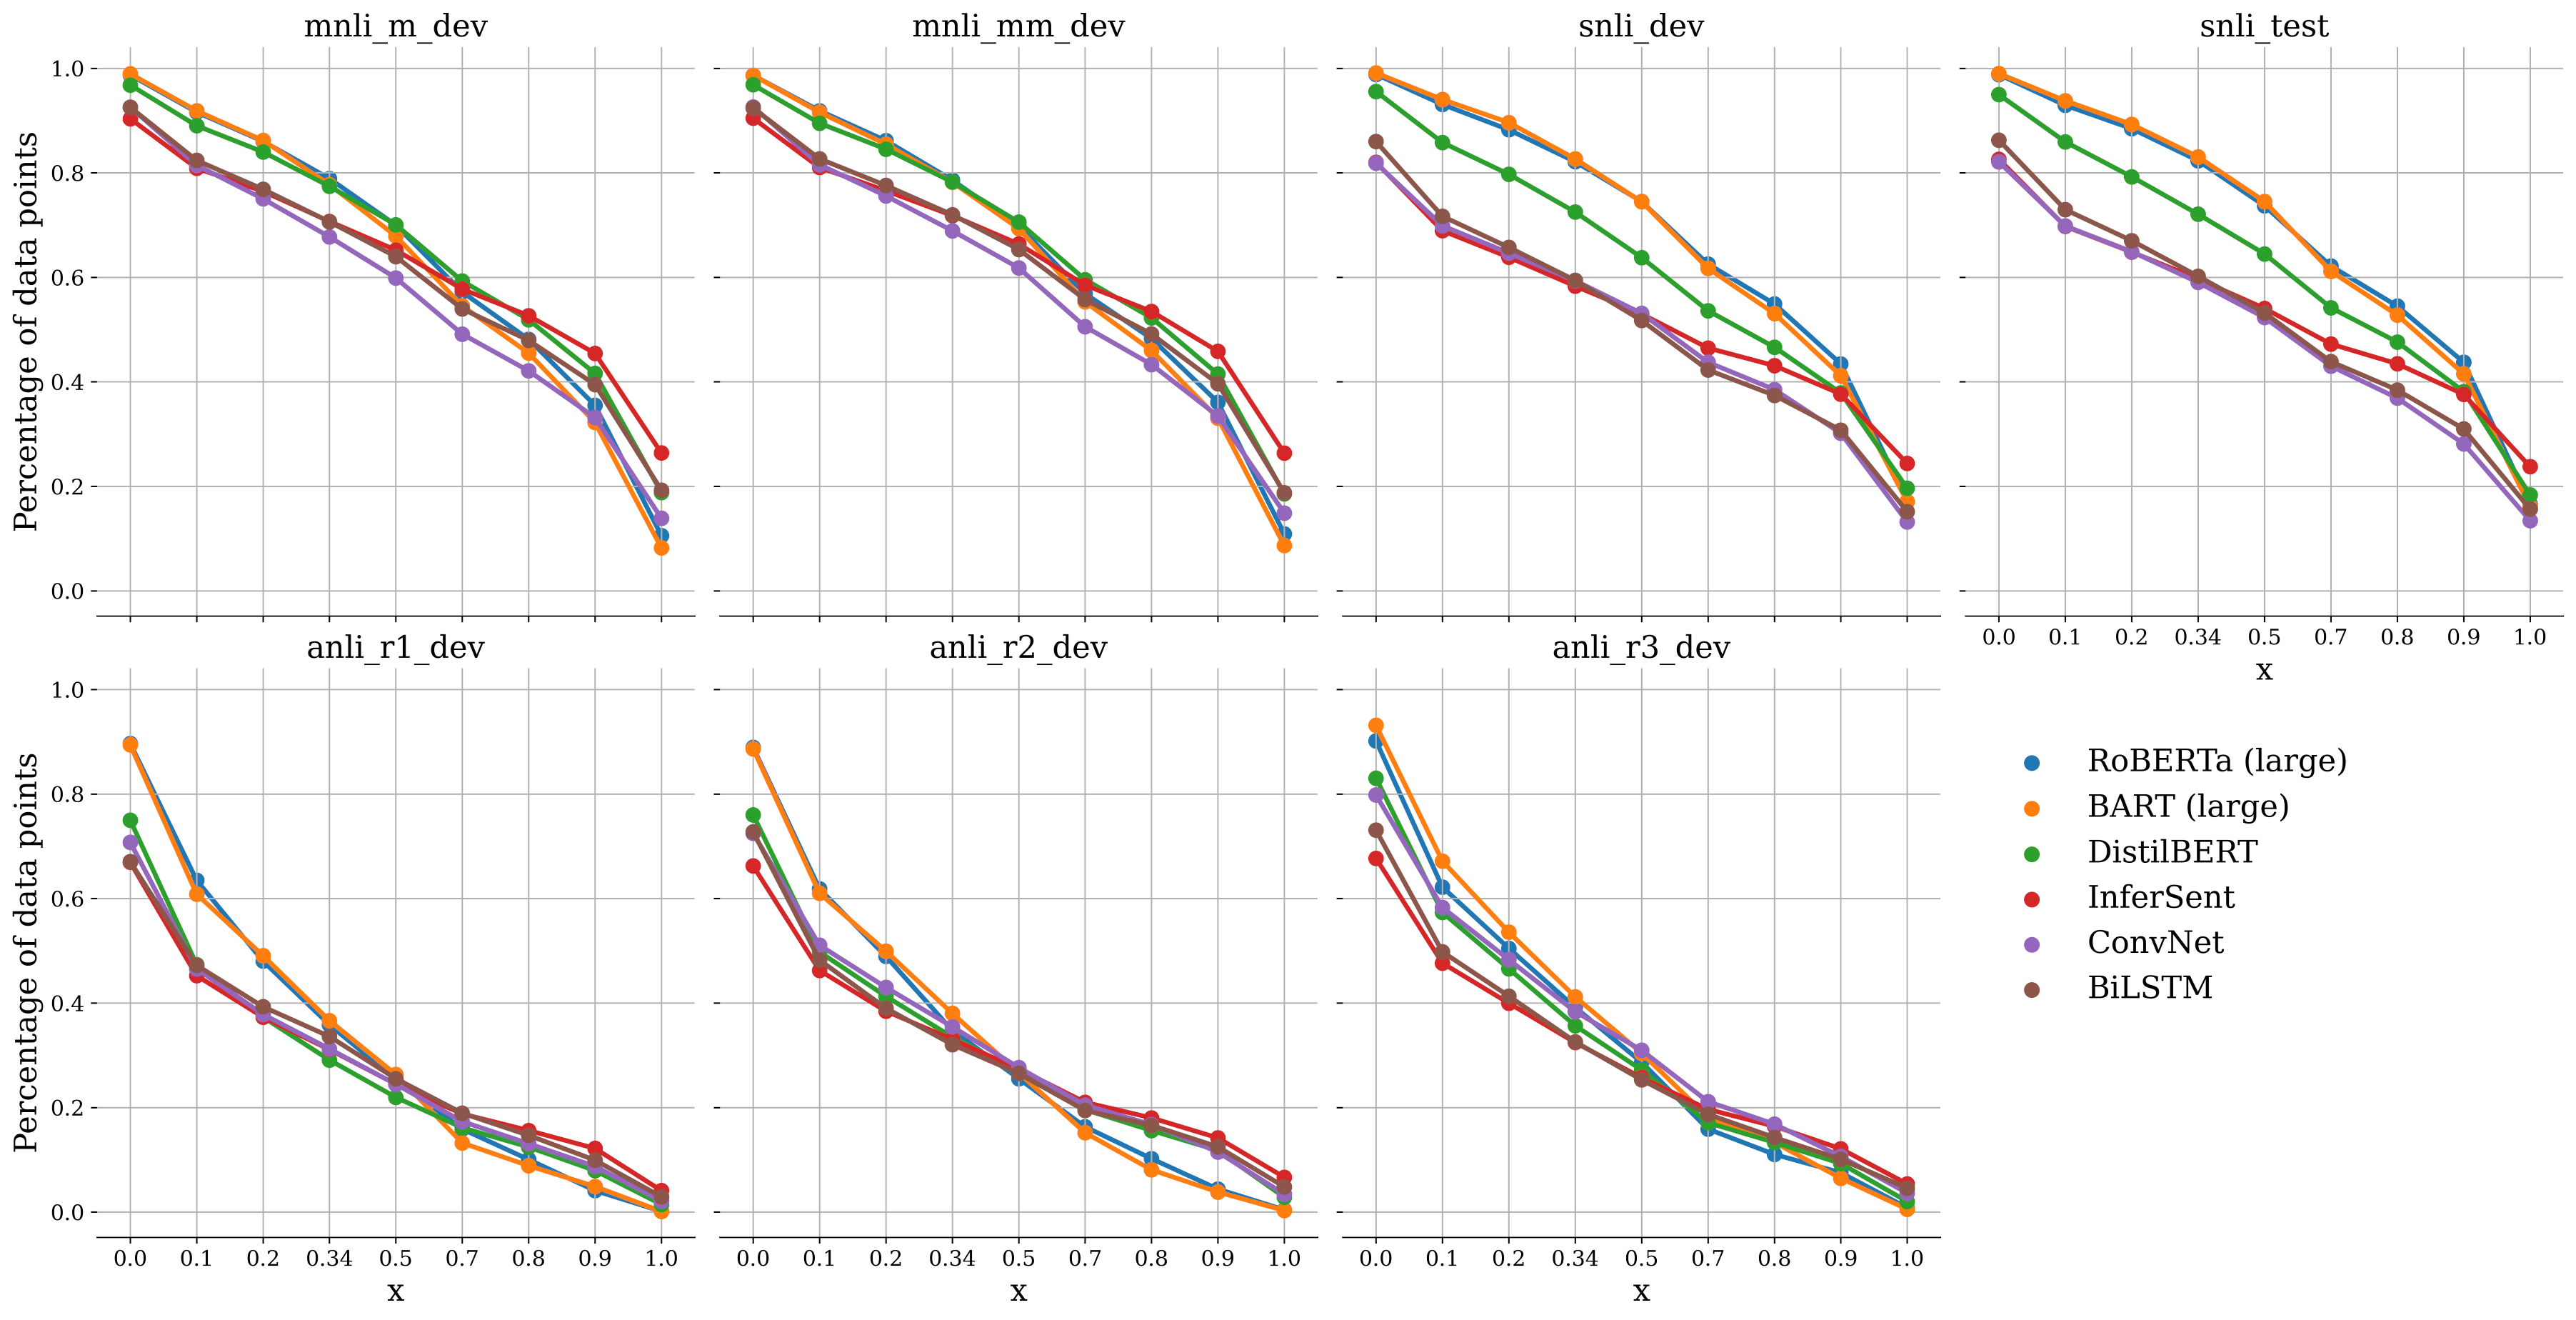
\includegraphics[width=.9\linewidth]{figs/unli/omega_threshold.png}
\caption{\(\omega_{x}\) threshold for all datasets with varying \(x\) and computing the percentage of examples that fall within the threshold.}
\end{figure}



\section{Related Work}
\label{sec:org90572c9}
\section{Discussion}
\label{sec:orgdd9c593}
\section{Follow-up findings in the community}
\label{sec:orgef6955a}

\clearpage
\chapter{Probing syntax understanding through distributional hypothesis}
\label{sec:org881cedf}

Paper: \cite{sinha2021}

\section{Technical Background}
\label{sec:org21235b5}
\section{Dataset construction and pre-training}
\label{sec:orgc04b18b}
\section{Experiments}
\label{sec:org987c7f3}
\subsection{Downstream reasoning tasks}
\label{sec:org3d7661e}

\begin{figure}[htbp]
\centering
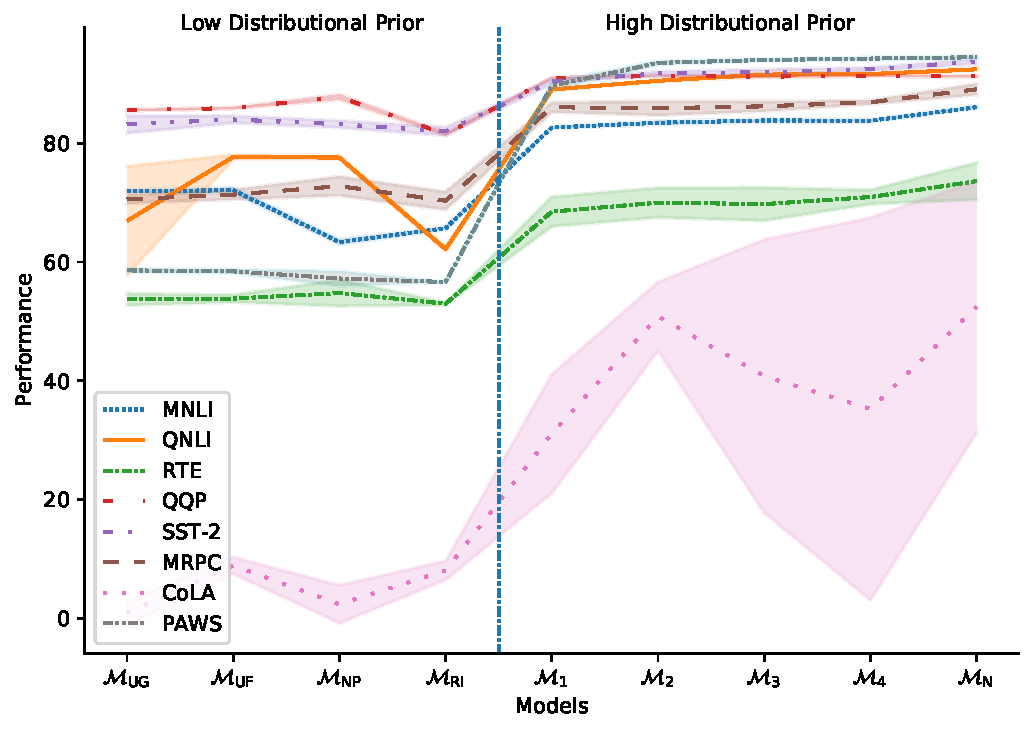
\includegraphics[width=.9\linewidth]{figs/unnat_pt/main_result_plot.pdf}
\caption{Downstream results on scrambled pre-training.}
\end{figure}

\begin{figure}[htbp]
\centering
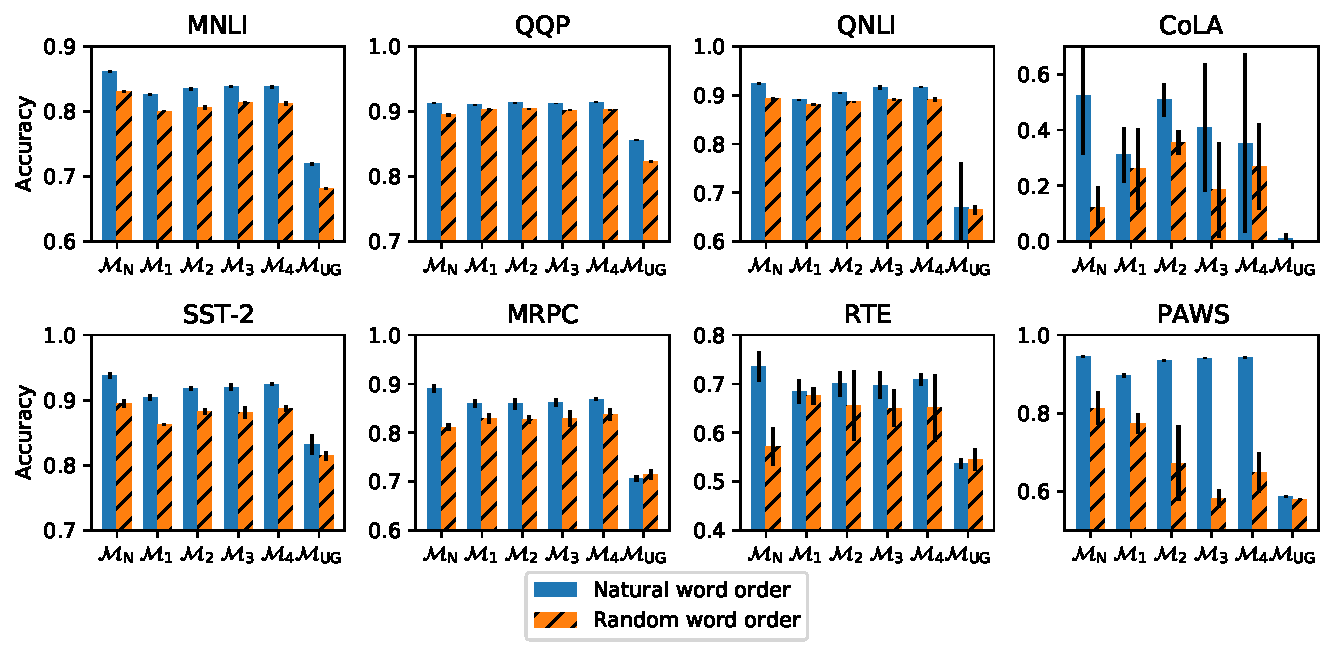
\includegraphics[width=.9\linewidth]{figs/unnat_pt/finetune_rand.pdf}
\caption{GLUE and PAWS task dev set performance when finetuned on naturally and randomly ordered text, respectively, using pre-trained RoBERTa (base) models on different versions of BookWiki corpus.}
\end{figure}

\subsection{Evaluating the effectiveness of probing syntax}
\label{sec:orgde81009}

\begin{figure}[htbp]
\centering
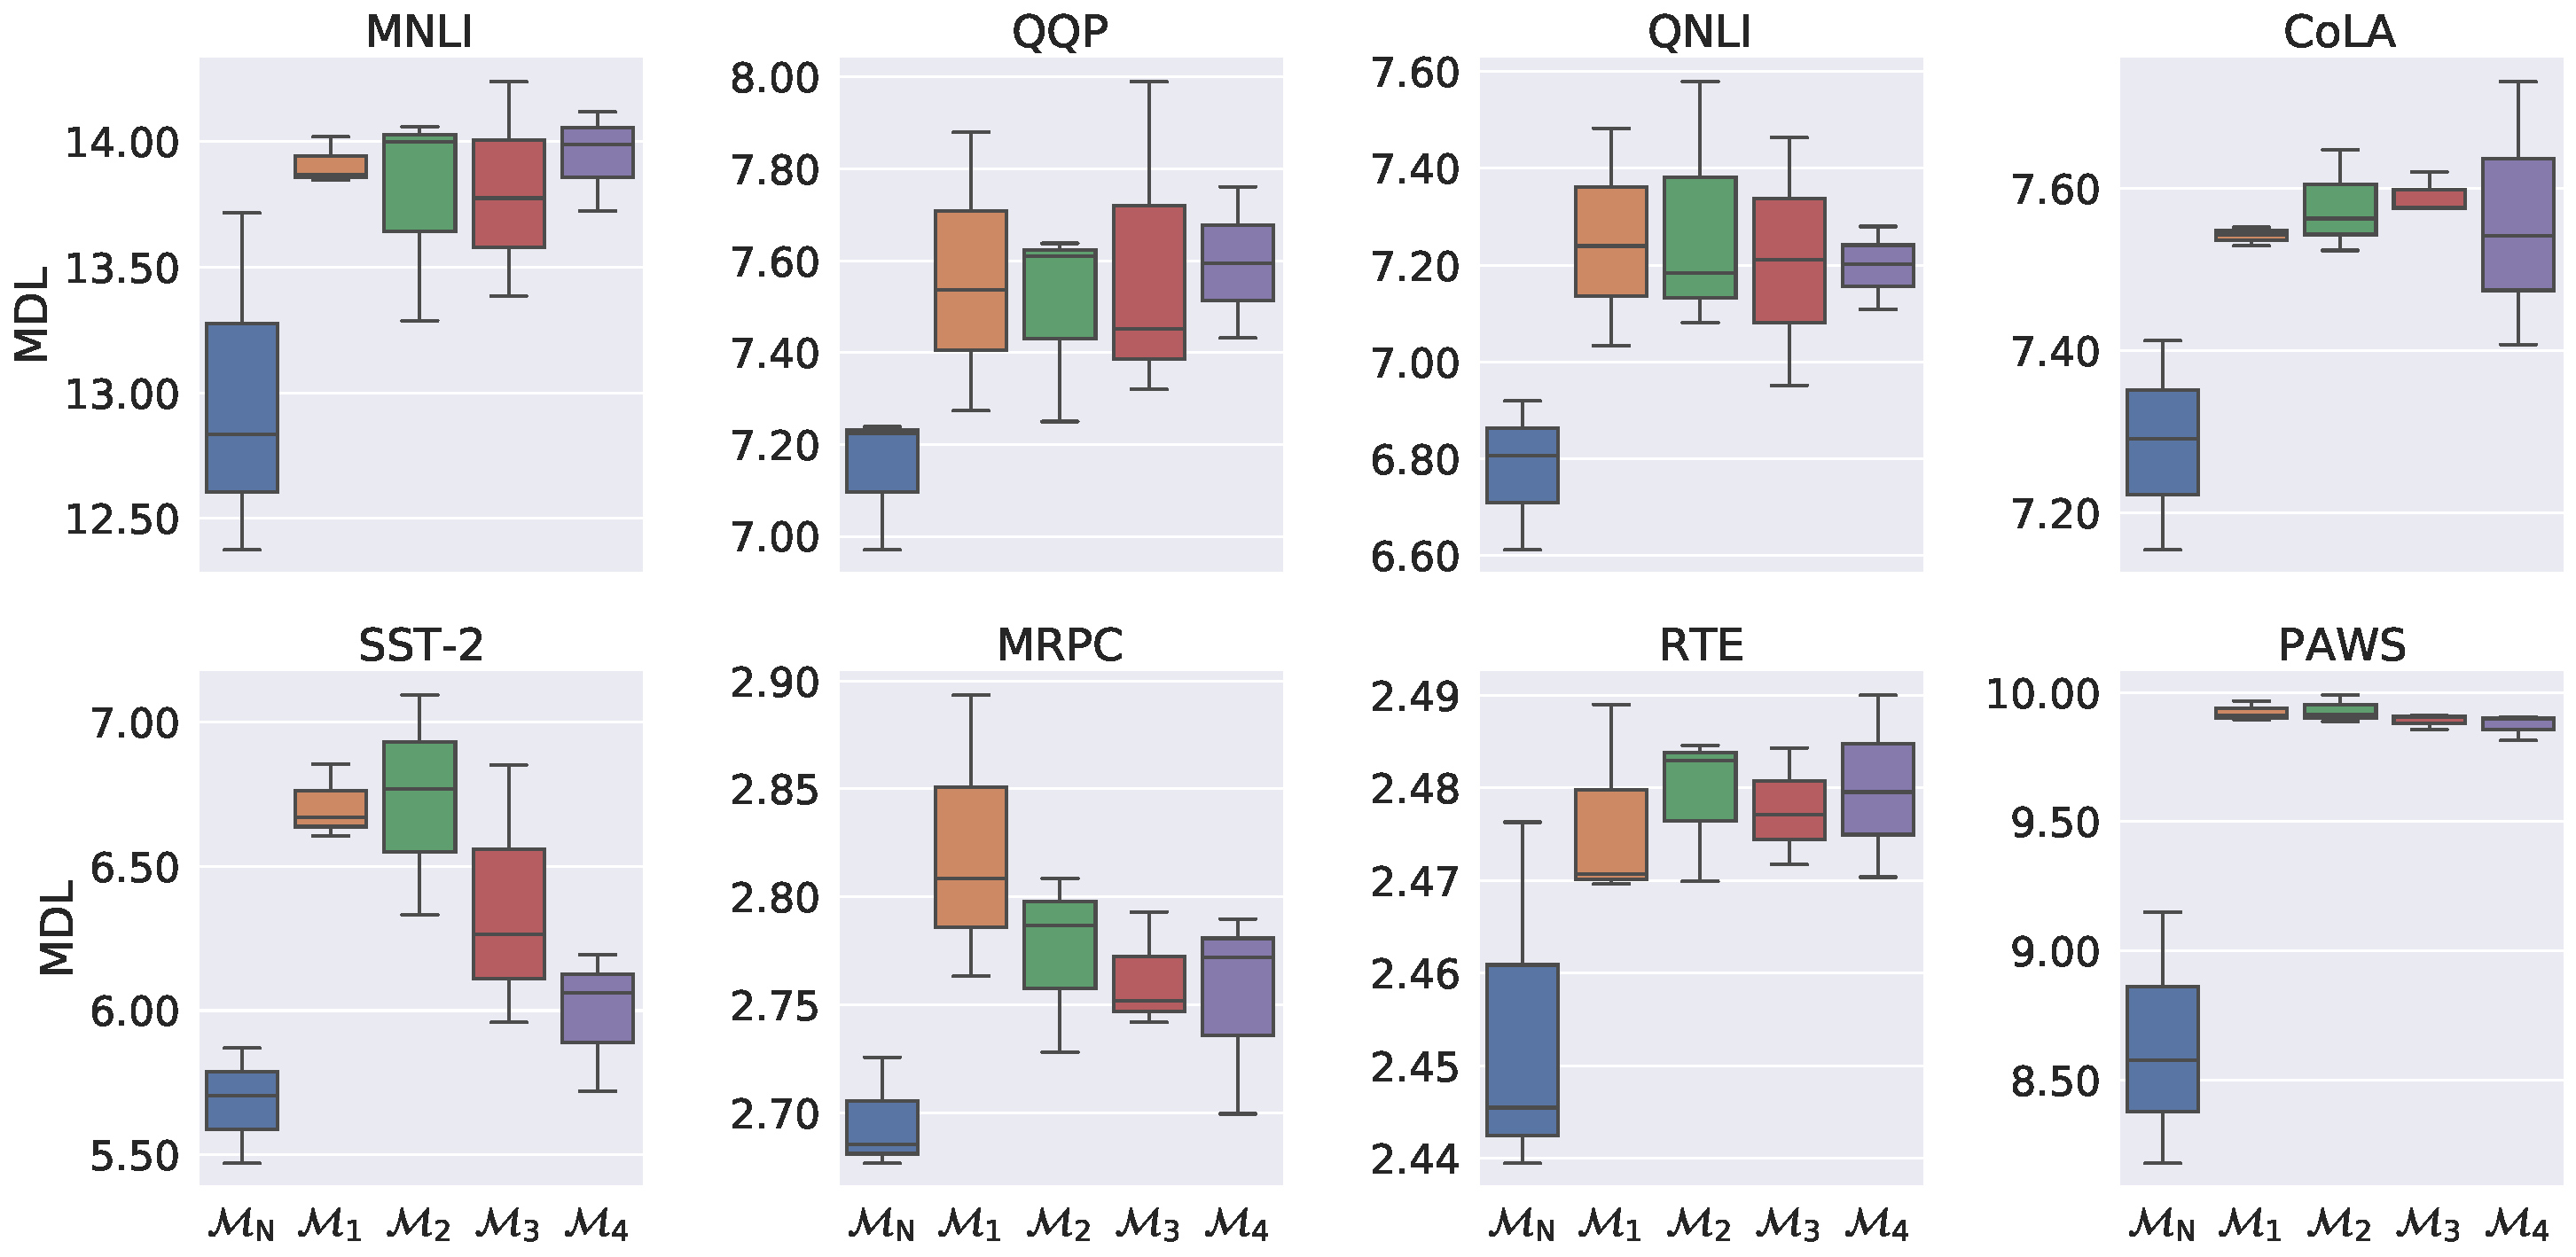
\includegraphics[width=.9\linewidth]{figs/unnat_pt/rda_mdl_ep_3.pdf}
\caption{Risannen Data Analysis.}
\end{figure}

\section{Related Work}
\label{sec:orgc510385}
\section{Discussion}
\label{sec:org25a2834}
\section{Follow-up findings in the community}
\label{sec:orgf893721}
\clearpage
\chapter{Measuring systematic generalization by exploiting absolute positions}
\label{sec:org4fe017f}

\section{Technical Background}
\label{sec:orge980475}
\section{Systematic understanding of absolute position embeddings}
\label{sec:orgc239d2d}
\section{Related Work}
\label{sec:org6149bb0}
\section{Experiments}
\label{sec:orgad6ec35}

\begin{figure}[htbp]
\centering
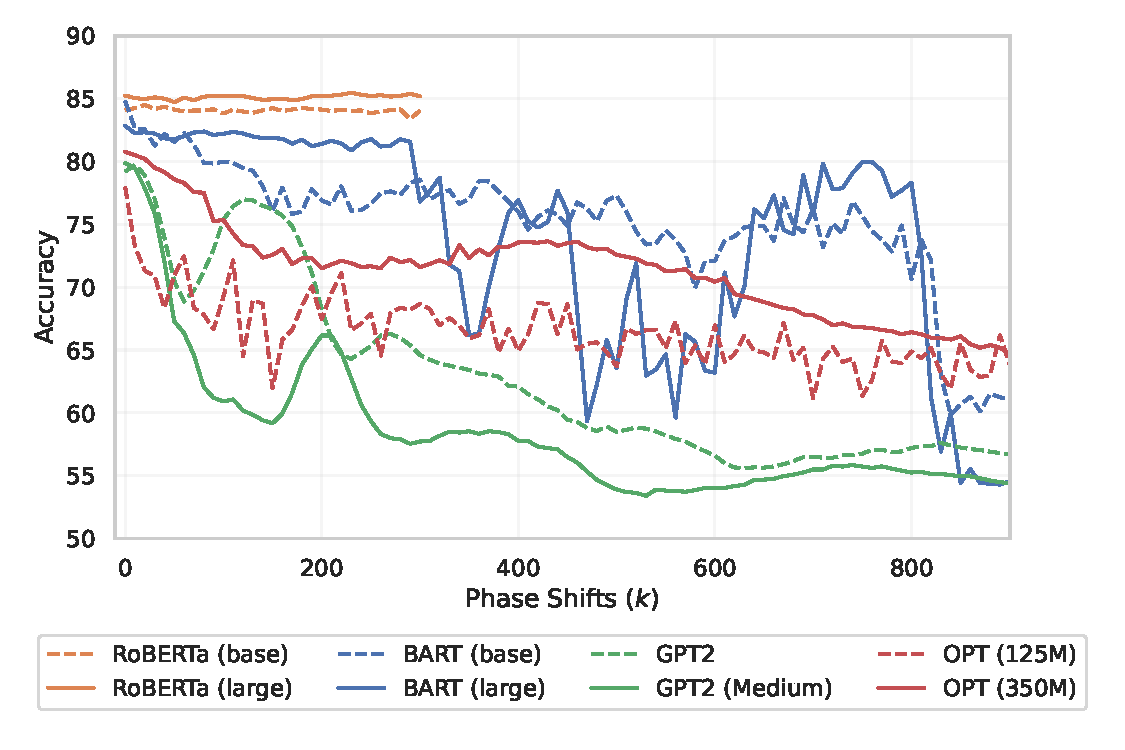
\includegraphics[width=.9\linewidth]{figs/pos_enc/acceptability_scores.pdf}
\caption{Grammatical acceptability scores on BLiMP dataset.}
\end{figure}

\section{Discussion}
\label{sec:org8d72560}
\clearpage
\chapter{Conclusion}
\label{sec:org0188af2}
\section{Summary}
\label{sec:org06f6c51}
\section{Limitations}
\label{sec:org338fd40}
\section{Future Work}
\label{sec:org67bf752}
\clearpage
\chapter{Bibliography}
\label{sec:org49a30b2}
\bibliographystyle{unsrt}
\bibliography{../../mylibrefs_new,bibfiles/unli,bibfiles/clutrr,bibfiles/pos_enc,bibfiles/unnat_pt,bibfiles/anthology}


\printglossaries

\chapter{Appendix}
\label{sec:orgfe900d8}
\section{Org mode auto save}
\label{sec:org9aa068f}
Run the following snippet to auto save and compile in org mode.

\begin{verbatim}
(defun kdm/org-save-and-export ()
(interactive)
(if (and (eq major-mode 'org-mode)
    (ido-local-file-exists-p (concat (file-name-sans-extension (buffer-name)) ".tex")))
  (org-latex-export-to-latex)))

(add-hook 'after-save-hook 'kdm/org-save-and-export)
\end{verbatim}

\section{Remove ``parts'' from report}
\label{sec:org9b6eddf}

\begin{verbatim}
(add-to-list 'org-latex-classes
             '("report-noparts"
               "\\documentclass[11pt]{report}"
               ("\\chapter{%s}" . "\\chapter*{%s}")
               ("\\section{%s}" . "\\section*{%s}")
               ("\\subsection{%s}" . "\\subsection*{%s}")
               ("\\subsubsection{%s}" . "\\subsubsection*{%s}")))
\end{verbatim}
\section{Add newpage before a heading}
\label{sec:org01683d7}

\begin{verbatim}
(defun org/get-headline-string-element  (headline backend info)
  (let ((prop-point (next-property-change 0 headline)))
    (if prop-point (plist-get (text-properties-at prop-point headline) :parent))))

(defun org/ensure-latex-clearpage (headline backend info)
  (when (org-export-derived-backend-p backend 'latex)
    (let ((elmnt (org/get-headline-string-element headline backend info)))
      (when (member "newpage" (org-element-property :tags elmnt))
        (concat "\\clearpage\n" headline)))))

(add-to-list 'org-export-filter-headline-functions
             'org/ensure-latex-clearpage)

\end{verbatim}

\section{Glossary and Acronym build using Latexmk}
\label{sec:orga3bc779}

Add the following snippet in the file ``\textasciitilde{}/.latexmkrc'': (Source: \url{https://tex.stackexchange.com/a/44316})

\begin{verbatim}
add_cus_dep('glo', 'gls', 0, 'run_makeglossaries');
add_cus_dep('acn', 'acr', 0, 'run_makeglossaries');

sub run_makeglossaries {
    my ($base_name, $path) = fileparse( $_[0] ); #handle -outdir param by splitting path and file, ...
    pushd $path; # ... cd-ing into folder first, then running makeglossaries ...

    if ( $silent ) {
        system "makeglossaries -q '$base_name'"; #unix
        # system "makeglossaries", "-q", "$base_name"; #windows
    }
    else {
        system "makeglossaries '$base_name'"; #unix
        # system "makeglossaries", "$base_name"; #windows
    };

    popd; # ... and cd-ing back again
}

push @generated_exts, 'glo', 'gls', 'glg';
push @generated_exts, 'acn', 'acr', 'alg';
$clean_ext .= ' %R.ist %R.xdy';
\end{verbatim}
\section{Citation style buffer local}
\label{sec:org61822fa}

\begin{verbatim}
(set (make-local-variable 'bibtex-completion-format-citation-functions)
  '((org-mode      . my/bibtex-completion-format-citation-org-default-cite)))
\end{verbatim}
\section{Org latex compiler options}
\label{sec:orgbba41e5}

\begin{verbatim}
(setq org-latex-pdf-process (list "latexmk -f -pdf -%latex -interaction=nonstopmode -output-directory=%o %f"))
\end{verbatim}

Original value

\begin{verbatim}
(setq org-latex-pdf-process (list "latexmk -f -pdf %f"))
\end{verbatim}

Let us try Fast compile \url{https://gist.github.com/yig/ba124dfbc8f63762f222}.

\begin{verbatim}
(setq org-latex-pdf-process (list "latexmk-fast %f"))
\end{verbatim}

\begin{itemize}
\item Doesn't seem to work from Emacs.
\item I need to change the save function to only export in tex. Then, have a separate process run latexmk.
\item Using the python package \texttt{when-changed} to watch the thesis.tex file for change.
\item Usage:
\end{itemize}

\begin{verbatim}
when-changed thesis.tex latexmk -f -pdf -interaction=nonstopmode -output-directory=%o thesis.tex
\end{verbatim}

\begin{itemize}
\item The pdf does not update. It seems to but not always? No it does. For some reason, compilation takes ages.
\item Works with \texttt{when-changed}!
\end{itemize}
\end{document}
